\documentclass[a4paper, 12pt]{extarticle}
\usepackage{polyglossia}
\setdefaultlanguage{ukrainian}
\setotherlanguage{english}

\usepackage{fontspec}
\setmainfont{CMU Sans Serif}
\newfontfamily{\cyrillicfonttt}{CMU Typewriter Text}

\usepackage[left=2.5cm, top=2.5cm, right=1.5cm, bottom=1.5cm]{geometry}

\linespread{1.5}
\setlength{\parindent}{0cm}

\usepackage{listings, color}
\definecolor{dkgreen}{rgb}{0,0.6,0}
\definecolor{gray}{rgb}{0.5,0.5,0.5}
\definecolor{mauve}{rgb}{0.58,0,0.82}
\lstset{
  frame=tb,
  language=Lisp,
  aboveskip=3mm,
  belowskip=3mm,
  inputencoding=utf8,
  extendedchars=\true,
  showstringspaces=false,
  columns=flexible,
  basicstyle={\small\ttfamily},
  numbers=left,
  numberstyle=\tiny\color{gray},
  keywordstyle=\color{blue},
  commentstyle=\color{dkgreen},
  stringstyle=\color{mauve},
  breaklines=true,
  breakatwhitespace=true,
  tabsize=2
}


\begin{document}

\begin{titlepage}
  \newgeometry{left=2.5cm, top=1.5cm, right=1.5cm, bottom=1.5cm}
  \thispagestyle{empty}
  \center
  \textsc{\uppercase{Міністерство освіти і науки України\\Національний технічний університет України\\<<Київський політехнічний інститут>>}}\\[1cm]
  \textsc{Кафедра обчислювальної техніки}\\[0.5cm]
  \vfill
  \textsc{\Large \textbf{Лабораторна робота \#1}}\\
  \textsc{з дисципліни}\\
  \textsc{\large ``Декларативне програмування''}\\
  \textsc{на тему:}\\
  \textsc{\Large <<Опис та виклик функцій у мові Lisp>>}\\
  \vspace{3cm}
  \begin{minipage}{0.4\textwidth}
    \begin{flushleft} \large
      \emph{Виконав:}\\
      студент гр. ІП-32 \\
      \textsc{Ковальчук О. М.} % Your name
    \end{flushleft}
  \end{minipage}
  \begin{minipage}{0.4\textwidth}
    \begin{flushright} \large
      \emph{Перевірив:} \\
      доцент каф. АСОІУ \\
      \textsc{Баклан І. В.} % Supervisor's Name
    \end{flushright}
  \end{minipage}\\[4cm]
  \vfill

  Київ 2015
\end{titlepage}
\setcounter{page}{2}
\section{Мета і задачі}
\textbf{Метою роботи} є вивчення базових функцій організації та обробки списків, а також способів опису і виклику нерекурсивних функцій у мові програмування Lisp
\textbf{Основні задачі}
\begin{itemize}
  \item Отримати навички роботи з інтерпретатором Lisp
  \item Вивчити роботу базових функцій із розширення набору примітивних функцій
  \item Ознайомитися з описом функцій у Lisp
\end{itemize}

\section{Визначення завдання}
\subsection{Визначення вихідних даних та індивідуального завдання}
Номер за списком --- 13. Отже, номер варіанту завдання --- 13.
Таким чином:

\textbf{Вихідні списки:}
\begin{itemize}
  \item (REM FFG HHJ (H )J G D)
  \item (2 34 56 78 (7 8))
  \item (UN Y LOOP)
\end{itemize}

\textbf{Номери елементів:}
\begin{itemize}
  \item \textit{Список 1:} 4
  \item \textit{Список 2:} 4
  \item \textit{Список 3:} 2
\end{itemize}

\textbf{Індивідуальне завдання:}
Дано списки, наприклад, '(1 2 3 4 5) та '(7 6 5 7). Якщо добуток перших елементів вихідних списків додатній, то у результуючий список слід об'єднати останні елементи заданих списків. Інакше --- скласти результуючий список із останнього елементу першого списку та хвоста другого.

\subsection{Завдання 1}
Описати неіменовану функцію для об'єднання голів трьох списків в один. Вихідні данні обрати згідно варіанту.

\subsection{Завдання 2}
Описати іменовану функцію для створення нового списку із елементів вихідних списків. Вихідні списки та номери елементів обрати згідно варіанту.

\subsection{Завдання 3}
Виконати індивідуальне завдання згідно варіанту.

\section{Виконання}
\lstinputlisting[caption=Визначення констант]{constants.lsp}
\lstinputlisting[caption=Неіменована функція]{task-01.lsp}
\lstinputlisting[caption=Іменована функція]{task-02.lsp}
\lstinputlisting[caption=Індивідуальне завдання]{task-03.lsp}
\lstinputlisting[caption=Об'єднання]{task.lsp}

\section{Результати}
\subsection{Завдання 1}
\begin{figure}[h!]
  \centering
  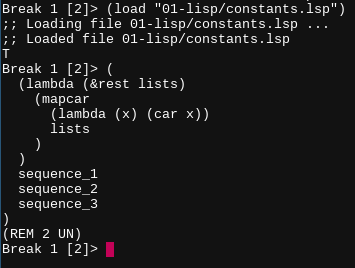
\includegraphics[width=0.5\textwidth]{screenshots/task-01.png}
\end{figure}
\subsection{Завдання 2}
\begin{figure}[h!]
  \centering
  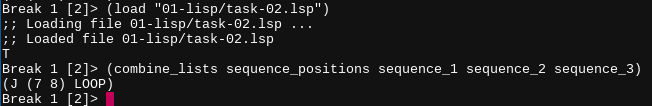
\includegraphics[width=0.9\textwidth]{screenshots/task-02.png}
\end{figure}
\subsection{Завдання 3}
\begin{figure}[h!]
  \centering
  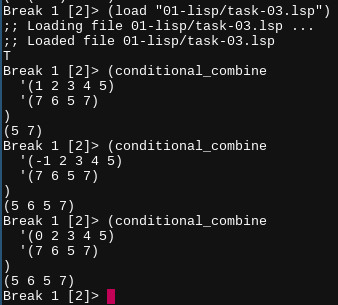
\includegraphics[width=0.5\textwidth]{screenshots/task-03.png}
\end{figure}

\end{document}
